\chapter{Design} % 

To recap, this project used a hybrid approach of a plan-driven methodology followed by an agile implementation. The design stage is where the first methodology began to merge into the other.

A lot of time was invested in clarifying requirements so that the common classes and methods could be established and fed into parts of the initial design. Certain design documentation, such as the database schema, was worth spending time creating and could be designed up front, since it was unlikely to change unless there was a change in requirements. Other things, such as class diagrams would not be suitable for upfront design, since the code would be refactored throughout the process and it would ultimately fall out of line with the documentation.

\section{Development choices}

\subsection{Programming language}

As a web-based solution, the options were somewhat constrained to server-side languages. PHP, Node and Ruby on Rails all came to mind. It was decided that PHP would be the most appropriate choice.

PHP is currently the most popular server-side programming language worldwide [REF], and, perhaps more importantly, it's the server-side language I have by far the most experience using. My philosophy was this: though I could have spent a few weeks learning the ins and outs of ASP.NET to deliver my project, it would be an unwise use of my time given that there was so much to build. I didn't want to find myself desperately trying to debug an obscure error in an unfamiliar language a week before the deadline. % http://w3techs.com/technologies/overview/programming_language/all

Development experience aside, PHP being the most popular server-side language means that there is extensive support and documentation online: any problems faced during development have likely already been solved by other peoples' experiences. Moreover, if the project were to go open-source, it would be more likely to acquire a sizeable and active developer community than a lesser-known language such as Go.

With my suite of Cucumber features, I needed a set of accompanying step definitions. The PHP de-facto standard implementation of BDD is Behat,  but after much lamenting on which BDD framework to use, I decided that the project should use Ruby and Cucumber as its BDD framework, primarily for its cleaner syntax but also to force decoupling between the core system and the end-to-end tests. See appendix~\ref{appendix:bdd} for a full justification.

\subsection{Reusing open-source software}

It was hoped that there would be an existing open-source ODR platform upon which to base the project. One would have been able to make the necessary modifications and extensions to support the maritime collision module, without having to build the entire platform from scratch, thereby being able to spend more time on the maritime law module.

Unfortunately, even after fairly extensive research (see appendix ~\ref{appendix:choosingAFramework}), I was unable to find an existing ODR platforms that was not proprietary. Most ODR providers, be they service or platform providers, charge a subscription or one-off fee and would be at a commercial disadvantage if they were to go open source.

Without an existing ODR platform to base the project upon, there was no option but to develop the core platform from scratch.

\subsection{Framework}

It makes sense to minimise development effort through the use of a framework, letting the combined efforts of hundreds of contributing developers do the heavy lifting so that we are free to implement the application-specific code. Dozens of PHP frameworks exist, so deciding on one can be difficult.

Large frameworks such as Zend and Symphony are very constraining, requiring you to stick to their idea of what is the best development approach (specific directory structures, MVC design pattern, and so on) or else perform some very heavy, non-standard configuration to make it suit your project. Either of these heavyweight frameworks could be perfectly well suited to ODR, but generally speaking I try to stay away from non-transferable frameworks. I like to understand exactly how my application works, rather than delegate that understanding to a third-party library, and I like having the freedom to change frameworks painlessly at a later date - something which is not suited to heavyweight frameworks.

Lighter options exist: these include Huge, Opauth, Laravel and Fat-Free Framework. Huge looked promising to begin with but then appeared to be more of a middleweight framework, strongly encouraging certain directory structures. It would be a base that the ODR software would have to build upon, rather than a library that could be plugged into the system, only called as and when needed.

Opauth looked nice and lightweight, but was aimed at projects which want to use OAuth for authentication, allowing people to sign in using their Twitter, Google, LinkedIn or Facebook account. This was not suitable, given our project requirements. Laravel was the next one considered and looked a little like PHP's answer to Rails, as it generates an entire application structure through a proprietary command.

Almost any one of the above frameworks would have been a suitable starting point. It would be impossible to thoroughly evaluate every framework to make a truly considered decision.

For me, the most promising framework at first glance was Fat-Free Framework, or F3 as it is commonly known, as it has a low learning curve and an unconstraining nature. Its modular build meant that I could cherrypick the elements of functionality needed for the project, rather than go for an all-or-nothing installation. Interaction with the library is almost entirely through calls to namespaced classes. F3 is fundamentally different to its competitors because I could slot F3 into my code, rather than slotting my code into F3. For these reasons, I chose F3 as SmartResolution's framework.

In a recent interview I presented this argument to Gavin Love, Chief Technology Officer at MyBuilder.com, who agreed that modularity seems to be the way that PHP frameworks are heading. This suggests that delegating units of functionality to a lightweight framework might be quite a wise, future-proof decision. Developing software on a heavyweight framework which subsequently loses support can be very difficult to refactor, as Gavin says he found when upgrading MyBuilder.com from Symphony 2 to Symphony 3.

\section{Overall architecture}

The project can be broken down into three main components:

\begin{enumerate}
    \item \textbf{Core platform}, AKA SmartResolution. The majority of the project was spent developing this ODR platform.
    
    \item \textbf{Maritime collision module}. This is a plugin for the SmartResolution software that defines a `Maritime Collision' dispute type and offers custom actions and business logic for these specialised cases.
    
    \item \textbf{SmartResolution Website}. The website should describe how to download and install the core platform. It should also offer a `marketplace' option to facilitate the download and installation of modules directly through a SmartResolution installation.
\end{enumerate}

\subsection{Core platform}

SmartResolution is the ODR platform offering the core online dispute resolution requirements, such as organisation and user registration, dispute creation, messaging, file uploads, and so on. It offers the minimum facilities necessary to successfully negotiate a dispute online.

As this will be the basis of all the other components, it should also be the most thoroughly engineered, backed up with integration and unit tests, continuous integration, automated code quality checks and dependency status checks.

\subsection{Maritime collision module}

This module is separate from the core platform and lives in its own repository [REF]. It can be installed to any SmartResolution installation simply by being copied to the \lstinline{modules} directory; no further configuration is required.

As discussed in the background and initial requirements, it was intended for this to be a feature-rich module that could find similar historic cases, cross-check agents' answers with maritime law, and approximate the likelihood of an agent's success in court.

\subsection{SmartResolution Marketplace}

This is the vendor site for SmartResolution, explaining what SmartResolution is and offering a download link to a production-ready version. Its subdomain, demo.smartresolution.org, has a live demo of the SmartResolution software installed so that users can try out the software before they download. However, the main purpose for smartresolution.org is the \emph{Marketplace} facility.

\section{WordPress: a comparison}

The commercial viability of the software (discussed in appendix~\ref{appendix:commercialViability}) drew some parallels with the blogging software WordPress. They could be said to have a three-tier system:

\begin{enumerate}
    \item \textbf{WordPress platform}: blogging software that can be downloaded, installed and hosted on your own server.
    
    \item \textbf{WordPress plugin}: a self-contained package that can be installed to a WordPress installation and augment the core installation with additional functionality.
    
    \item \textbf{Plugin Directory}: a searchable area of the WordPress.org website, accessible directly through your own WordPress installation, allowing the painless and automatic installation of plugins. This facility is tightly coupled to the administrative functions in the core software. Administrators are able to browse, download and install plugins from wordpress.org, from within the WordPress installation itself. % https://wordpress.org/plugins/
\end{enumerate}

These three tiers map to the SmartResolution core platform, the maritime collision module and the SmartResolution Marketplace respectively.

Some developers can be quite snooty about WordPress, but it is a platform that powers 23\% of the internet.[REF] The reasons for this are that it is open source, customisable with a choice of thousands of themes and plugins, and the developer documentation is very good. The brand is reliable: people trust it. I will try to emulate all of this as much as possible in the development of SmartResolution. % http://w3techs.com/technologies/details/cm-wordpress/all/all

\section{Choice of Licenses}

The design section may seem an incongruous place to discuss the issue of licensing, but licensing is just a very high-level form of design. Linus Torvalds, chief architect of the Linux kernel, once said he considered his choice of the GPL ``one of the very best design decisions" he made when developing the kernel, since it is designed to protect the author's legal and moral rights to their code. Moreover, the choice of license for each component in this project highlights how distinct each component is from one another, emphasising the need for a separate design, implementation and testing strategy for each of the components. % http://www.linuxjournal.com/article/2736

I opted for the GPLv3 license [REF] for the core SmartResolution software. This is almost identical to WordPress' choice of a GPLv2 license, which is presumably still at version 2 for legacy or backwards-compatibility reasons.

The benefits of a restrictive license such as the GPL licenses is that nobody has the ability to download, modify and then sell the software without making the source available to all. Big companies, who should compensate developers for their time, are not able to use SmartResolution as a basis for closed-source software. Any improvements they make to the software must be kept open-source, as it is a derivative work.

On the other hand, legitimate use-cases for SmartResolution are perfectly allowed. For instance, anyone can download the software and install it on their own server and start providing ODR services, perhaps even for a subscription fee. There's no requirement to suddenly make everything on their website open-source, as they are not distributing their website, only the \emph{results} of the server-side logic on their website (i.e. the HTML). The Affero GPL license (AGPL) would be a different story, as it closes this distribution-over-a-network loophole. [REF]

To summarise, the choice of GPLv3 for SmartResolution protects me from other people making money selling \emph{software} derived from this project. It doesn't stop people making money providing ODR as a service, and it doesn't ``infect their website like a cancer", to paraphrase Steve Ballmer, ex-CEO of Microsoft. [REF]

In stark contrast to my choice of license for SmartResolution, I've released the maritime collision module under the MIT license, which is the most permissive license available. I wanted developers to be able to download and modify this module as a basis for their own modules, and I want developers to be excited about the commercial opportunity SmartResolution presents for them. If they were to base their module on the maritime collision module, and if that module were bound to the terms of the GPL, they would be obliged to release the source code of their new module. This would make selling their module for a price implausible.

Modules do not have to be bound to SmartResolution's GPLv3 license because they do not alter the core functionality of the system. They are not derived works of the system. They are simply self-contained applications which, it could be argued, `just happen' to work when copied into a particular directory in SmartResolution.

Finally, I have kept the source-code for smartresolution.org private and all of its contents are under my copyright. I saw no advantage in making the website open source, since I'm not encouraging anybody to download and re-use elements of the website itself. All in all, the three components of my project are covered by three very different licenses.

\section{Design: SmartResolution}

\subsection{Choice of Database Management System}

The first decision to be made was whether to go for a traditional relational database management system (RDBMS) or an object-oriented database management system (OODBMS). The former is the traditional means of application persistence. The latter is still fairly new, and is intended to allow developers to think purely in terms of object-orientation and not worry about mapping object-oriented paradigms to a relational database.

Though I considered using the latter, there is more widespread support for the former, and I wanted SmartResolution to be as accessible as possible for those wanting to provide their own ODR services. My choice of PHP framework, F3, has built-in database support and is geared towards relational databases, though also provides an object-relational mapping layer [REF] as a compromise between the two paradigms. %http://fatfreeframework.com/databases#CRUD(ButWithaLotofStyle)

OODBMSs gives an advantage to those companies that are geared towards multimedia presentation or organizations that utilize computer-aided design. [REF] In contrast, SmartResolution is quite text-heavy and is perfectly well suited to a RDBMS implementation. % O'Brien, J. A., & Marakas, G. M. (2009). Management Information Systems (9th ed.). New York, NY: McGraw-Hill/Irwin

My next decision was which RDBMS to go for. The market leader is MySQL [REF], but many alternatives exist, such as PostgreSQL, MSSQL, Oracle and SQLite. F3 supports all of these and more. [REF] %http://fatfreeframework.com/sql#Constructor

The quickest database to get started with was SQLite, as it meant that I could develop locally and wouldn't have to install other programs, such as MySQL or PHPMyAdmin. It exists simply as a file on the system, and its contents can be viewed and edited through a program such as DB Browser for SQLite [REF]. %http://sqlitebrowser.org/

The fact that SQLite databases exist as files on the system makes having multiple databases trivial, so my system can easily switch between test and production databases depending on the context in which the application is accessed.

For these reasons, I selected SQLite as the RDBMS of choice for the project. It is important to note that this can be swapped out for another RDBMS relatively easily, since all database interactions in SmartResolution go through one \lstinline{Database} class. This class calls F3's \lstinline{SQL} class, and as discussed above, F3 has implementations for all of the main RDBMSs. Consequently, my choice of RDBMS isn't a critical decision.

For a SmartResolution installation that is in a production environment and is being used by hundreds or thousands of people, I would consider changing to a RDBMS such as MySQL. Even the SQLite developers suggest that SQLite is well suited as a ``stand-in for an enterprise RDBMS. SQLite is often used as a surrogate for an enterprise RDBMS for demonstration purposes or for testing". [REF] %https://www.sqlite.org/features.html

\subsection{Database schema}

\begin{figure}[h!]
  \centering
    \ifimages
    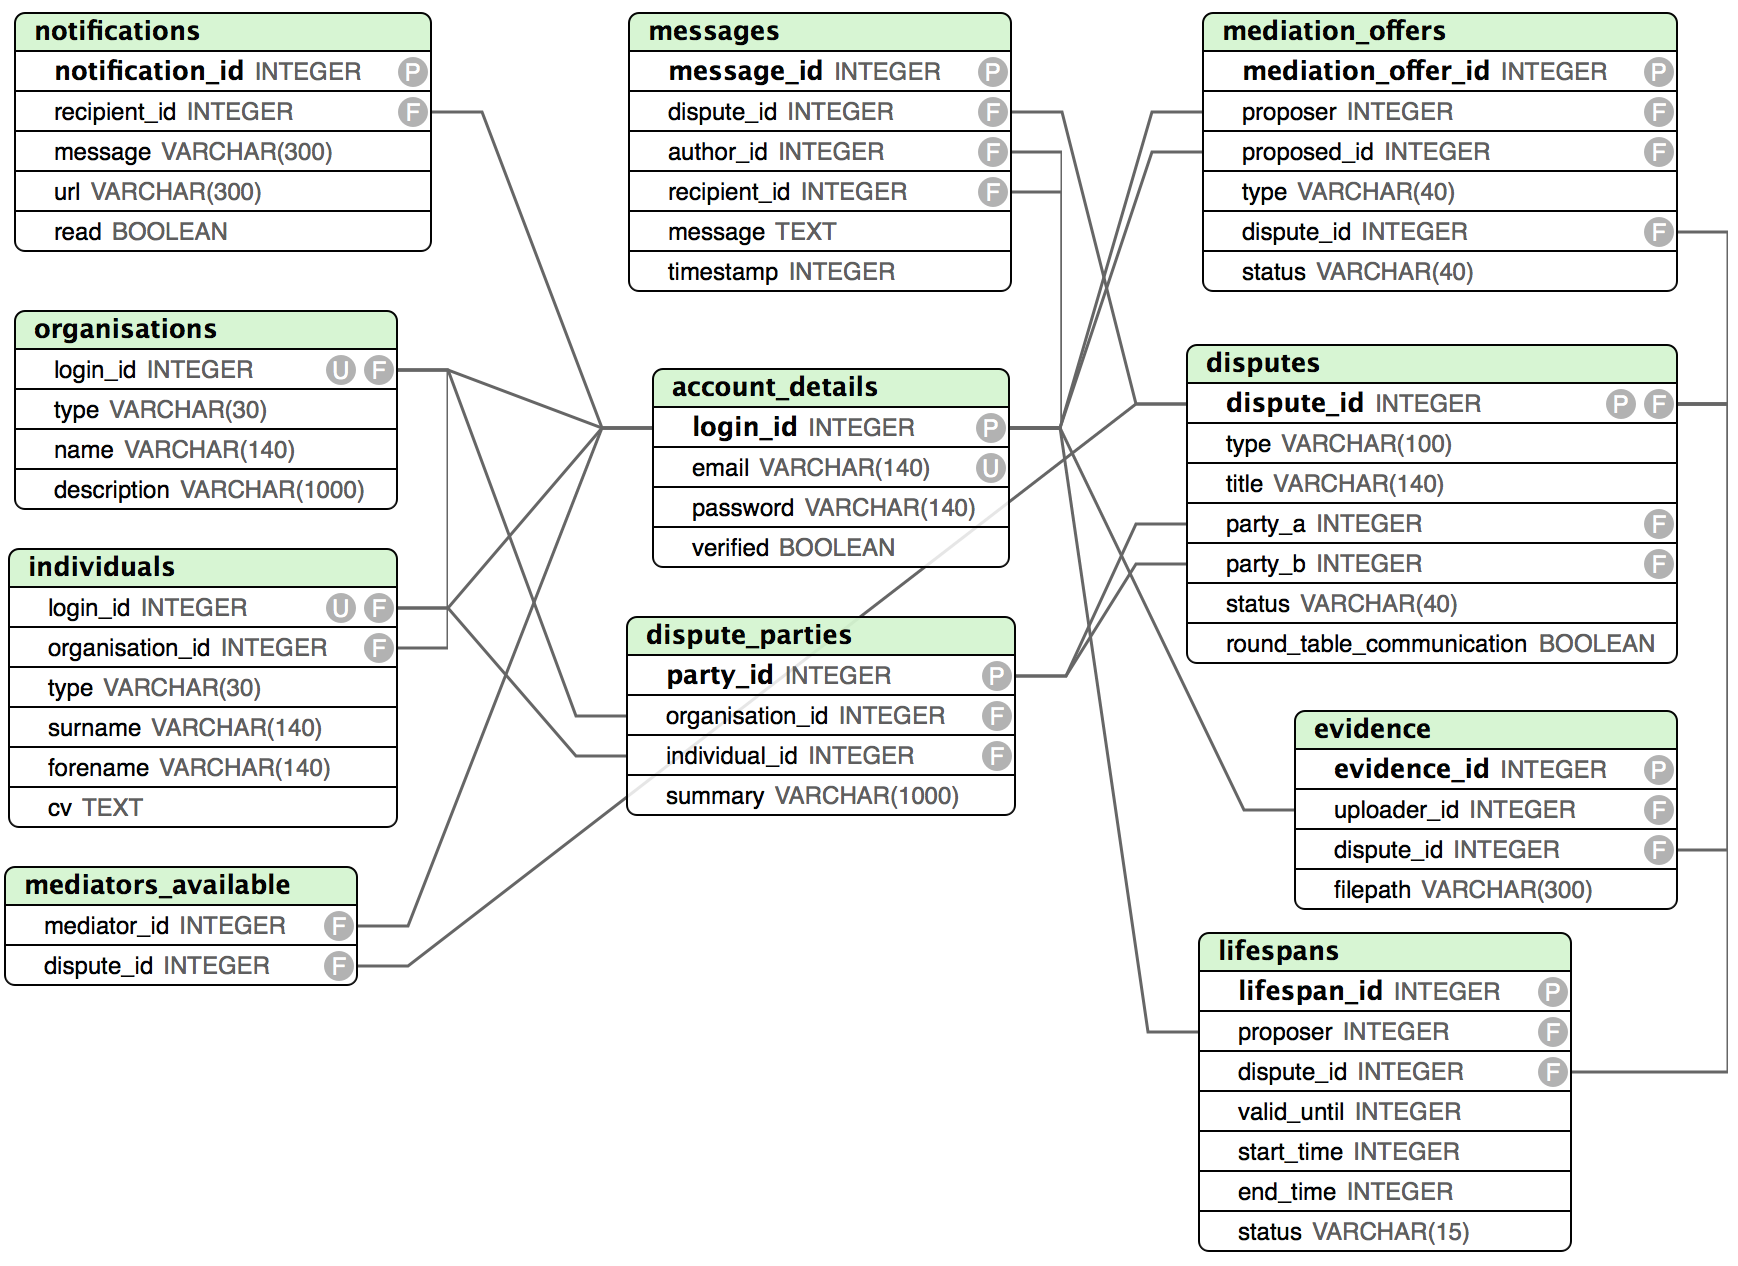
\includegraphics[width=\textwidth]{database}
    \fi
  \caption{Database schema for the SmartResolution core platform}
  \label{uml:databaseSchema}
\end{figure}

Figure~\ref{uml:databaseSchema} shows the database schema for the SmartResolution core platform, where \lstinline{P} symbols refer to primary keys, \lstinline{F} symbols refer to foreign keys, and \lstinline{U} symbols refer to unique integrity constraints. Lines generally denote where one table key references another, i.e. a foreign key visualisation.

Other integrity constraints exist, such as `organisations.type' only being one of ``law\_firm" or ``mediation\_centre". These have been omitted from the diagram.

For a full explanation and justification of the database design, please refer to appendix~\ref{appendix:database}.

\subsection{Module support}

This section of work is separate from the maritime collision module work, and is concerned with how the core platform should support modules at an abstract level. There should be no maritime-collision-specific code in the core SmartResolution platform, but the platform must support all functionality required by the module.

Taking inspiration from WordPress' Plugin API, the project uses the concept of `hooks'. WordPress fires events at various points throughout the normal running of a WordPress installation; these events can be subscribed to and a custom function executed to achieve some arbitrary purpose.

For example, below is the \lstinline{add_filter} function [REF]: %http://codex.wordpress.org/Function_Reference/add_filter

\begin{lstlisting}
add_filter('img_caption_shortcode', 'my_img_caption_shortcode_filter',10);
\end{lstlisting}

The first argument is the event to listen for, the second argument is the custom function to execute, and the third argument is an integer denoting the priority of our subscription, where a higher integer means our custom function is executed before subscribing functions of a lower-priority. SmartResolution fires hooks which can be subscribed to in the same way as the WordPress function above.

F3's routing API [REF] can extend this route-handling concept further:

\begin{lstlisting}
$f3->route('GET /some-route' => 'MyClass->handler');
\end{lstlisting}

F3's routing allows the developer to assign handling to a public method of a class, rather than a global function, keeping the codebase namespaced and tidy. This is something I've carried over to SmartResolution's parsing of the function name.

These principles formed the basis for the design of the module support:

\begin{lstlisting}
on('event', 'function_to_call', 'priority');
\end{lstlisting}

`event' is the name of the event to subscribe to, `function\_to\_call' is the name of the function to call (and can be a global function, a named class function or an anonymous function), and `priority' represents the priority with which the function should be called. It can be an integer or a string such as `high', `medium' and `low'.

\subsection{Exposing other methods}

An event-subscription mechanism can only get you so far. One needs to be able to manipulate the rendered output of SmartResolution, for example adding a menu item to the dashboard of a dispute.

This could be accomplished by interacting with the core platform, as in the example below.

\begin{lstlisting}
global $dashboardActions;
$item =  array(
    'title' => $params['title'],
    'image' => $params['image'],
    'href'  => $params['href']
);
array_unshift($dashboardActions, $item);
\end{lstlisting}

However, this encourages tight coupling between the module and the underlying platform, locking the core platform into a particular design and risking breaking backwards compatibility should SmartResolution be refactored in the future. For example, if the \lstinline{$dashboardActions} global variable was removed from the core platform, or the dashboard actions represented with something other than an array, it could break any existing modules relying on that specific implementation.

Again, WordPress provided inspiration for the design. WordPress exposes a number of global functions, e.g. \lstinline{get_the_id}, which gets the ID of the current post. [REF] In this style, SmartResolution exposes a number of global functions. [REF] One could now manipulate the rendering of the dashboard like this: % %https://codex.wordpress.org/Function_Reference/get_the_ID
% http://smartresolution.org/module-docs/index.html

\begin{lstlisting}
dashboard_add_item(array(
    'title' => 'Some Action',
    'image' => get_module_url() . '/images/icon.png',
    'href'  => get_dispute_url() . '/custom-route'
));
\end{lstlisting}

Not only does this decouple the module/SmartResolution interaction, but this is much cleaner and easier from the module developer's perspective. It is important that there should be as few barriers as possible when it comes to module development, if developers are to get excited about SmartResolution.

\subsection{Module persistence}

This was the most difficult area to tackle, as it raises important security issues. Whereas hooking into events and changing the rendering could break aspects of the SmartResolution functionality if the developer is not careful, these are usually temporary and reversible. Interacting with the database, however, introduces persistent changes and can do much more damage.

If the system allowed arbitrary SQL queries and an uncareful developer accidentally executed a \lstinline{DROP TABLE} statement, all manner of data could be lost. This isn't so important on a small demo site with three or four registered users, but if SmartResolution were ever used on a large-scale website, the result could be catastrophic.

On the one hand, the system has to trust developers. Regardless of the database access explicitly exposed, there's nothing stopping a developer from running PHP's \lstinline{shell_exec} function [REF] and executing any command they wish. Also, in terms of the database interaction, there's nothing stopping developers from accessing the global \lstinline{Database} class used by the core platform, especially since SmartResolution is open source and the developer can easily find out what system-level classes are available.

The system should trust developers, but it should not trust developers to write perfect code. Though most developers would use an SQL-execution ability only for querying the database for a legitimate reason, they may expose a vulnerability if not thoroughly tested. For example, if they're writing a search engine module which takes a user input and if they do not sanitise the query, then they're letting the \emph{end user} run arbitrary SQL.

With security in mind, it was decided that the global function definitions should be expanded to define functions supporting specific SQL interactions, e.g. creating tables, selecting rows, updating records, and so on. Early on it was tempting to allow table schema updates on the fly, creating columns as and when they were needed, but this felt dangerous and was tricky to implement. I settled on an up-front table design solution by way of a \lstinline{declare_table} function:

\begin{lstlisting}
declare_table('my_table', array(
    'a_text_field' => 'TEXT NOT NULL',
    'an_int_field' => 'INTEGER DEFAULT 0',
    'initiated'    => 'BOOLEAN'
));
\end{lstlisting}

This could then be inserted into and queried using specific, named functions. This does somewhat restrict what the developer can do - for example, there is no method for doing SQL table joins - but more often than not, the developer can still achieve what they need to achieve using pure application code.

In the above example, \lstinline{my_table} is not the name of the created table. Instead, it is namespaced as \lstinline{module__[module_name]__my_table}. The module developer doesn't need to know this, and can continue to refer to \lstinline{my_table} in all of their queries as if that is the name of the table. This means we have the advantage of namespacing our tables (preventing duplicate table names between modules for common table names, e.g. ``config") but without the technical overhead of having to rememember to prefix table names with that namespace.

Most modules will require some sort of persistence layer to be useful, but developers are not necessarily locked into this database setup. They can use PHP's \lstinline{shell_exec} command to create a new SQLite database in their module's directory, giving them complete freedom and the responsibility it comes with. Or, they can use PHP's \lstinline{file_put_contents} to save to a file, perhaps in conjunction with \lstinline{json_encode} to save a PHP array as a JSON file. The database functions offered by SmartResolution cut out some of the complexity of doing this from scratch, but are by no means the only way of storing data persistently.

\section{Design: SmartResolution Marketplace}

Early versions of SmartResolution used a PHP array to describe which modules were installed and which were active. [REF] % https://github.com/ChrisBAshton/smartresolution/blob/6287211d49006e87a8d2035906eb58da22217906/webapp/modules/config.php 

A more user-friendly solution was the creation of an admin dashboard: the ability to sign into an administrator account on your SmartResolution instance, view the installed modules, and activate/deactivate them through a user interface. Following on from this is the ability to view a list of modules, pulled in from SmartResolution.org, and download and install them directly through SmartResolution, like WordPress does with plugins.

To accomplish this, there is a JSON feed of featured modules on smartresolution.org. [REF] This feed is pulled in and converted to HTML, both directly on the marketplace itself [REF] and the SmartResolution admin marketplace dashboard option, emulating what WordPress does with its modules (which are viewable both through your own installation of WordPress and on WordPress itself [REF]). %http://smartresolution.org/marketplace/feed
%http://smartresolution.org/marketplace
%https://wordpress.org/plugins/

From the admin dashboard on SmartResolution, the modules JSON feed is converted into a HTML page, and server-side logic detects whether or not the module is already installed on the instance. If not, an option is rendered to download and install the module in one button press.

In addition to the `Marketplace' admin option, there is a `Modules' option which lists all of the installed modules and whether or not they are active. From this screen, the admin can activate, deactivate or delete the module from their SmartResolution instance.

The ability to define which modules to display externally on smartresolution.org gives the SmartResolution maintainers the freedom to change the contents of that JSON, and therefore change which modules are presented to administrators of SmartResolution installations, regardless of when the instance was installed. This presents a commercial opportunity, allowing smartresolution.org to categorise paid-for modules as `featured', as hinted by the ``Coming soon" modules for Divorce and Breach of Contract.

\section{Design: Maritime collision module}

This module was developed in tandem with the module support in the core platform. As such, it uses most of the events and hooks exposed by the platform.

As discussed in the requirements section, the basis for the business logic in this module would be the Convention for the Unification of Certain Rules of Law with respect to Collisions between Vessels. Everything that is required to apply the Convention can be gathered from a few simple questions, visualised in the flowchart in figure~\ref{uml:maritimeLogic}.

\begin{figure}[h!]
  \centering
    \ifimages
    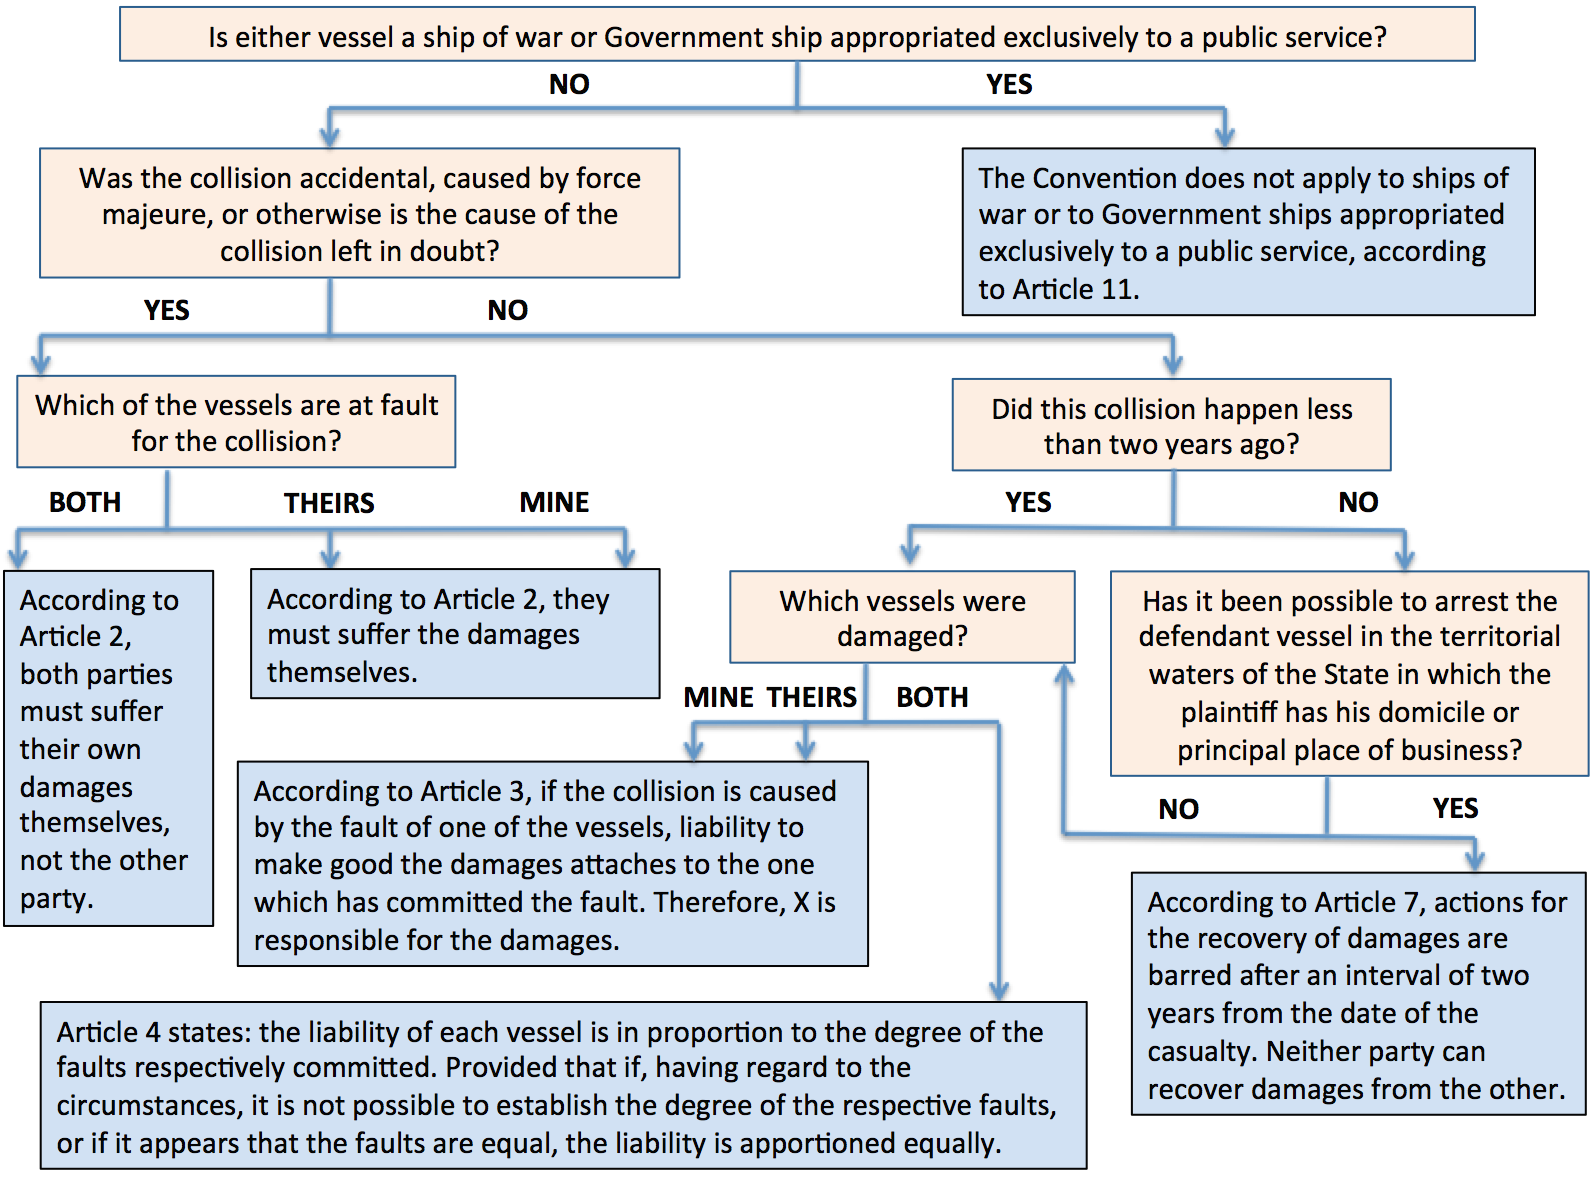
\includegraphics[width=\textwidth]{maritime_collision_logic}
    \fi
  \caption{Logic for Maritime Law results}
  \label{uml:maritimeLogic}
\end{figure}

Some of the business logic could be encapsulated in the JSON representing the questions. For example, some questions should only be displayed if certain prerequisites are satisfied. The questions are represented in the following format:

\begin{minipage}{\textwidth}
\begin{lstlisting}
    {
        "prerequisites": [
            {
                "question_id":     "article_11",
                "required_answer": "no"
            }
        ],
        "id":   "article_1",
        "text": "Which vessels were damaged?",
        "type": "select",
        "options": [
            {
                "text" : "The vessel of my client",
                "value": "mine"
            },
            {
                "text" : "The vessel of the other party",
                "value": "other"
            },
            {
                "text" : "Both vessels",
                "value": "both"
            }
        ]
    }
\end{lstlisting}
\end{minipage}

In the above example, the question whose id is \lstinline{article_1} (corresponding to Article 1 of the Convention) is only displayed if the agent answers the question whose id is \lstinline{article_11} with the answer ``no".

When the agents have answered all of the relevant questions, the following happens:

\begin{itemize}
    \item The answers are compared to make sure they tally. If one agent says both vessels were damaged and the other agent says only their vessel was damaged, the answers do not correspond and a conclusion cannot be reached. The module cannot be expected to cope with conflicting information. The module would inform the agents of this.
    \item Provided both answers correlate, the module's \lstinline{ResultsCalculator} class calls the \lstinline{deduceSummary} method [REF], which contains the hard-coded maritime law logic. A resolution is then presented to the agents.
\end{itemize}

Due to the lack of time, the resulting module is a little simplistic. The resolution suggested by the module is deduced through an ugly but simple series of if/else statements, and probably doesn't tell lawyers anything about maritime law that they don't already know.

However, over-examination of the maritime collision module would be missing the point, which is that the core platform supports any arbitrary module. Modules can be as big and complex as time allows. To go back to the WordPress analogy, on one end of the scale there are many one-script plugins that satisfy a lone developer's personal itch. On the other end, there are enterprise-level plugins that have taken months to engineer and which extend the WordPress platform to be a feature-rich online shop or forum. Given more time, the maritime collision module could be much more heavyweight than it is, encompassing many more aspects of maritime law.

\section{User interface}

Bootstrap was used to set up much of the initial design defaults and also provides basic UI framework for the layout. Bootstrap has a 12-column layout requiring a specific HTML structure and class-naming convention, but it does mean that the theme is fully responsive by default.

The CSS overrides provide a clean and attractive look, and helper classes such as \lstinline{bg-info} and \lstinline{bg-danger} allowed me to style error messages and other components with minimal effort, meaning I could spend more time on the server-side logic.